\begin{center}

  \begin{tabular}{rp{16cm}lp{20cm}}%{rl}

  % after \\: \hline or \cline{col1-col2} \cline{col3-col4} ...

  论文地址:& \href{https://arxiv.org/pdf/2101.05974.pdf}{https://arxiv.org/pdf/2101.05974.pdf} \\
  来源:& ICLR, 2021 \\
  作者:& Yanbang Wang, et al. \\

  源码:& \href{https://github.com/snap-stanford/CAW}{CAW} \\

%  slides:& \href{http://yunshengb.com/wp-content/uploads/2017/03/nips_2018_r2l_workshop_talk.pdf}{{\footnotesize Convolutional Set Matching for Graph Similarity}}\\

  关键词:& \textbf{Link Prediction, Causal Anonymous Walk, Temporal Graph} \\

  写于:& \date{2021-03-09}

  \end{tabular}

\end{center}

该论文\cite{wang2021inductive}就动态网络的模式抽取问题,针对现有方法中的一些弊端:如主要依靠结点id和丰富的边的属性且难以抽取复杂的模式,提出了CAW(Cusal Anonymous Walk)以inductive的形式表示动态图。CAW也是一种游走,在Temporal networks中以anonymization的策略游走生成CAWs,将这些CAWs作为motifs来表示动态网络。CAWs不需要传统的基于核方法中的选择什么样的motifs、统计motifs个数不同。再者,论文中提出了神经网络模型CAW-N用于编码CAWs。

\paragraph{问题定义}
动态网络中存在众多的模式,例如三角闭包以及一些更复杂的模式,目标就是在动态网络的表示中能够包含这些复杂的模式。当前对与动态网络的表示只能表示一些简单的模式或者主要停留在静态网络上。对于动态网络的研究主要由三个挑战:1)动态网络中结构和时序的混合,需要一个更好的模型对动态网络进行建模;2)模型的伸缩性,动态网络会不断地被新到来的数据更新;3)能够学习训练数据中出现过的数据,并提取出它的模式。

这里介绍一下inductive和transductive:Transduction is reasoning from obeserved, specific (training) cases to specific (test) cases. In contrast, induction is reasoning from obeserved training cases to gerneral rules, which are then applied to the test cases.

论文中用$\mathcal{E}=\{(e_1, t_1), (e_2, t_2), ...\}$表示动态网络,其中的含义显然易见。这个序列的边就编码的网络的动态性,那么,\textbf{动态网络的表示模型的表示能力就取决于能否准确地基于以往的信息预测结点之间的连接}。论文中也使用链接预测来作为模型的指标。

再介绍一些用到的符号:$\mathcal{E}_{v, t}=\left\{\left(e, t^{\prime}\right) \in \mathcal{E} \mid t^{\prime}<t, v \in e\right\}$表示在$t$之前与$v$相连的边集;下式表示一个CAW,注意其中时间使从大到小的,及新的边放在前面,$W[i]$表示第$i$个结点-时间对。
$$
W=\left(\left(w_{0}, t_{0}\right),\left(w_{1}, t_{1}\right), \ldots,\left(w_{m}, t_{m}\right)\right), t_{0}>t_{1}>\cdots>t_{m},\left(\left\{w_{i-1}, w_{i}\right\}, t_{i}\right) \in \mathcal{E} \text { for all }
$$

\paragraph{CAW思路}
在CAW之前有Anonymous walks(AW)\cite{micali2016reconstructing},如Fig.\ref{fig:aw}所示,AW很像随机游走,但是又与之有点不同 --- 用结点在walks中出现的顺序替代结点的id。这里也给我一个较大的启示:\tbc{red}{实践中对结点的编号并不能体现graph中的模式,在学习模式的表征时,应尽可能将实践时引入的编号等一些辅助信息与graph的结构、模式等区分开来。但是在实践时有时需要一个明确的表示的,可以借助一个中间的表示,将在不同应用场景下的表示转化为中间表示,用中间表示来表示模式。这有点类似于虚拟机和神经机器翻译中的概念}。
\begin{figure}[h]
	\centering
	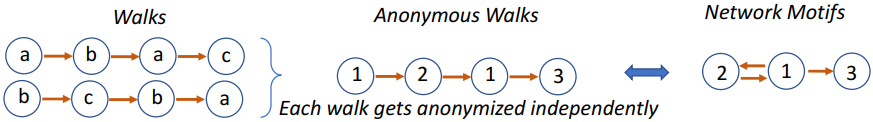
\includegraphics[width=.8\textwidth]{pics/AW.png}
	\caption{Anonymous walks}
	\label{fig:aw}
\end{figure}

CAW中就采用了这种思想,将结点的编号用结点在某个特定位置出现的次数代替。对于给定的两个结点,当预测它们的边时,需要先分别以这两个结点为起点抽取CAWs,再用论文中的方法替换结点的编号,再分别对walks进行编码,最后在预测边的概率。论文中提出的CAW-N主要由以下这些部分组成。
\subparagraph{Causal Anonymous Walk}
\textbf{Causal Anonymous Walk}由两部分组成:\textbf{Causality Extraction}和\textbf{Set-based Anonymization},如Fig.\ref{fig:caw}所示。

\begin{figure}[h]
	\centering
	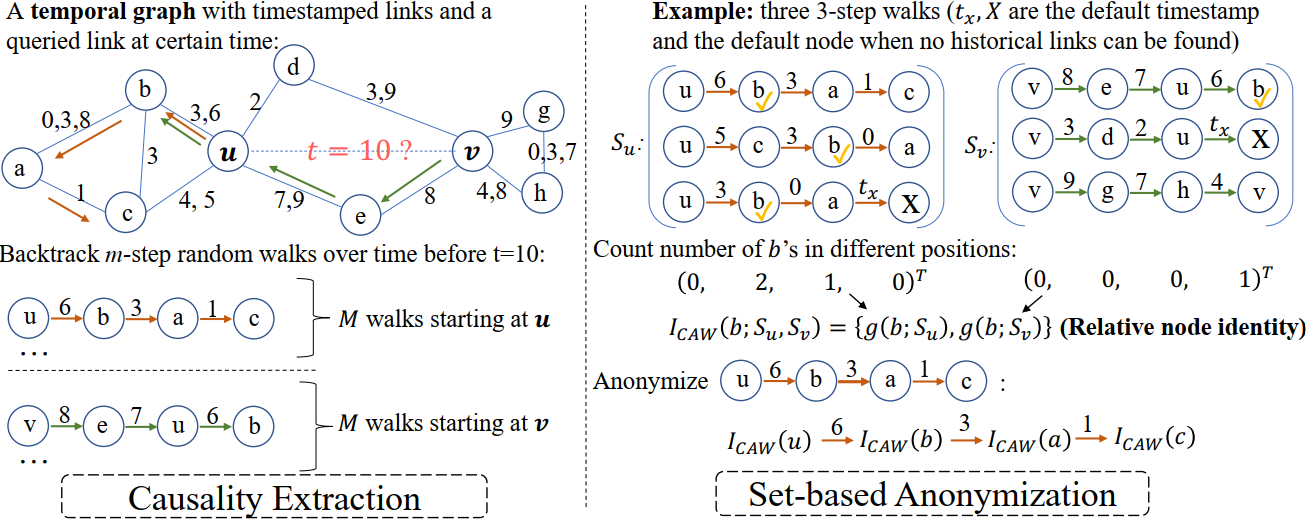
\includegraphics[width=.8\textwidth]{pics/CAW.png}
	\caption{CAW}
	\label{fig:caw}
\end{figure}

Causality Extraction这一部分主要用于从动态网络中抽取出walks(这个时候还不能称为Causal Anonymous Walks),抽取算法如Fig.\ref{fig:caw-walk-eatraction}所示。
\begin{figure}[h]
	\centering
	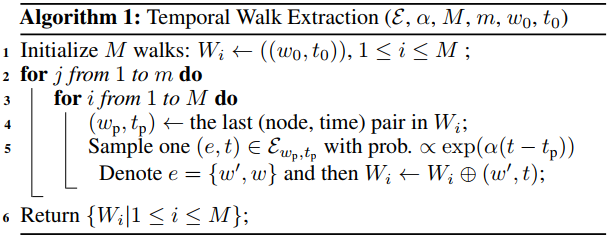
\includegraphics[width=.75\textwidth]{pics/CAW-Walk-Extraction.png}
	\caption{Temporal Walk Extraction}
	\label{fig:caw-walk-eatraction}
\end{figure}
对于结点$u_0, v_0$,该算法会分别以$u_0, v_0$为起点得到长度为$m$的$M$条CAWs,分别为$S_u, S_v$。得到walks后,需要将中的结点id去掉,转化成“中间表示”。转换过程就由Set-based Anonymization完成。

这一部分就是将walks中的结点id $w$转化为相对结点id $I_{CAW}(w; \{S_u,S_v\})$。\cite{micali2016reconstructing}中只是基于一条路径进行转换,这是基于一个假设:任意两个AWs不会共享结点id。显然,该论文中的转换是基于$2M$条CAWs转换的,这也是基于一个假设:\textbf{CAWs之间的关系可能是动态图中模式的关键之处}。因此共享结点id的CAWs就相当于保留了这种关系。$I_{CAW}(w; \{S_u,S_v\})$定义如下。
$$
I_{C A W}\left(w ;\left\{S_{u}, S_{v}\right\}\right) \triangleq\left\{g\left(w, S_{u}\right), g\left(w, S_{v}\right)\right\}
$$
对于$w_0 \in \{u, v\}$,$g(w, s_{w_0}) \in \mathbb{Z}^{m+1}$表示$w$在集合$S_{w_0}$中各个位置出现的次数。于是对于每一个walk可以表示为:
$$
\hat{W}=\left(\left(I_{C A W}\left(w_{0}\right), t_{0}\right),\left(I_{C A W}\left(w_{1}\right), t_{1}\right), \ldots,\left(I_{C A W}\left(w_{m}\right), t_{m}\right)\right)
$$

\subparagraph{Neural Encoding for Causal Anonymous Walks}
这一步是利用神经网络模型对$\hat{W}$进行编码,再将所有编码后的$\hat{W} \in S_u \cup S_v$聚集起来。

\par{\textbf{Encode $\hat{W}$}}文章采样的方法是将walk中的每个元素先进行编码,再输入到序列模型中,如下:
$$
\operatorname{enc}(\hat{W})=\operatorname{RNN}\left(\left\{f_{1}\left(I_{C A W}\left(w_{i}\right)\right) \oplus f_{2}\left(t_{i-1}-t_{i}\right)\right\}_{i=0,1, \ldots, m}\right), \text { where } t_{-1}=t_{0}
$$
其中$f_1, f_2$分别是$I_{CAW}(w_i), t_{i-1} - t_i$的编码函数,$f_2$就相当于\cite{tgat_iclr20}中的time encoding。$f_1$的实现可以是一个MLP,如$f_1(I_{CAW}(w_i)) = MLP(g(w_i, S_u)) + MLP(g(w_i, S_v))$。

\par{\textbf{Encode $S_u \cup S_v$}}
这一步就是聚集各个walk的encoding作为$S_u \cup S_v$的encoding来进预测$u, v$之间边的概率。论文中给出了两种参考的聚集方式:
\begin{itemize}
	\item Mean-AGG($S_u \cup S_v$): $\frac{1}{2M} \sum_{i=1}^{2M} enc(\hat{W})$
	\item Self-Att-AGG($S_u \cup S_v$): $\frac{1}{2M} \sum_{i=1}^{2M} softmax(\{enc(\hat{W_i}^T) Q_1 enc(\hat{W_j})\}_{1 \le j \le n}) enc(\hat{W_i}) Q_2$,其中$Q_1, Q_2 \in \mathbb{R}^{d \times d}$
\end{itemize}
再将$S_u \cup S_v$的encoding输入到MLP中进行预测。

论文中还提到了如何扩展模型使之能够融入结点/边的属性,将属性拼接到$enc(\hat{W})$的输入即可。


\paragraph{方法解决的问题/优势}

\begin{itemize}

	\item 提出了一个新的动态网络的表征模型CAW-N,能够对temporal network motifs进行编码,且该模型是inductive的
	\item 提出了一种新的方法来将walks转换到一个中间的表示空间
	\item CAWs不仅保留了网络中的temporal-spatial结构,还保留了motifs之间的关系,能够捕捉更复杂的模式

\end{itemize}



\paragraph{方法的局限性/未来方向}

\begin{itemize}

	\item 论文中只针对连接预测进行了实验,不知道在其他任务如结点分类等任务上效果怎么样
	\item 实验中对walk的长度取的都比较小,这样提取到的模式可能是比较短期的,较简单的模式

\end{itemize}



